\input format.tex

\usepackage{graphicx}
\graphicspath{{cores/}}

\usepackage{environ}
\usepackage{colortbl,array,booktabs}
\usepackage{tabularx}

\colorlet{TablaBordeSuperior}{topcolor}
\colorlet{TablaBordeInferior}{topcolor}
\colorlet{TablaCentroSuperior}{blue!1}
\colorlet{TablaCentroInferior}{blue!20}
\colorlet{FuenteCabeceraTabla}{white}

\newcolumntype{M}[1]{>{\centering\arraybackslash}m{#1}}
%\newcommand{\tabularxcolumn}[1]{>\arraybackslash}m{#1}}

\tcbset{rtab/.style={
freelance,
frame code={
 \path[top color=topcolor,bottom color=topcolor]
   ([yshift=-#1*(\baselineskip+2pt)]interior.north west) --
   ([yshift=-#1*(\baselineskip+2pt)]interior.north east) {[sharp corners]--
    ([yshift=3pt]interior.north east) --
    ([yshift=3pt]interior.north west)} -- cycle;

  },
interior code={},
 }
}

\newcommand\fuentecabecera[1]{\textcolor{black}{\textbf{#1}}}

\begin{document}

\vspace*{5mm}
%% 各章节
\setlength{\arrayrulewidth}{.2pt}
\fontsize{9.3pt}{11pt}\selectfont
\color{gray2}

{\noindent\bf\sanhao 三、相关疾病风险}

\begin{spacing}{1.5}
\begin{LRaside}[.8]{\fontsize{12pt}{11pt}\selectfont 检测说明}
\noindent
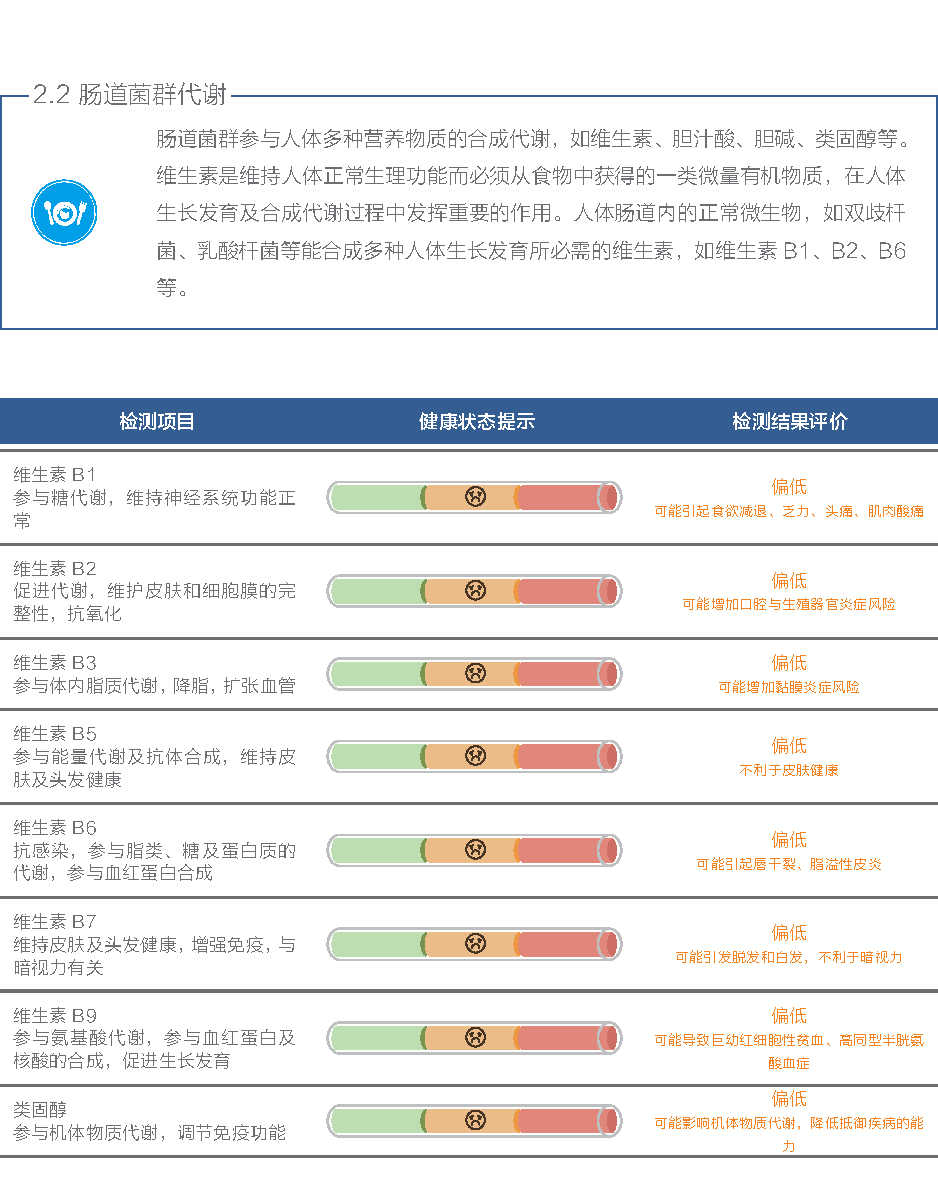
\includegraphics[width=\linewidth]{yingyanggongneng.pdf}
\asidebreak %
居住在人体肠道内的微生物菌群,不仅能够合成多种人体生长发育所必需的维生素、调节机体免疫力等,还与结直肠癌、炎症性肠病、高血压等数十种疾病密切相关。因此,
通过肠道菌群检测有效预测潜在疾病风险,真正实现了早检测早预防。
\end{LRaside}
\end{spacing}

\noindent 检测结果

\begin{tctabularx}{tabularx={m{4cm}<{\centering}m{6.6cm}<{\centering}m{4cm}<{\centering}}}
&&
\\[-6pt]
\cellcolor{topcolor} \raisebox{2.614pt}{\color{gray0}\bf 检测项目} &
\cellcolor{topcolor} \raisebox{2.614pt}{\color{gray0}\bf 健康状态提示} &
\cellcolor{topcolor} \raisebox{2.614pt}{\color{gray0}\bf 检测结果评价}
\end{tctabularx}

\vspace*{-4.25mm}
\fontsize{8.8pt}{11pt}\selectfont
\arrayrulecolor{gray2}
\begin{longtable}{m{4cm}<{\centering}m{6.6cm}<{\centering}m{0cm}@{}m{4cm}<{\centering}}

\hline
%\parbox[c]{\hsize}{\vskip7pt {\lantxh 结直肠癌\\ \bahao HASH(0x2e8ea58)} \vskip7pt} 
\parbox[c]{\hsize}{\vskip7pt {\lantxh 结直肠癌} \vskip7pt} & \parbox[c]{\hsize}{\vskip7pt\centerline{\raisebox{-1.5ex}{
\includegraphics[width=5cm,height=0.55cm]{diseasebar.pdf}}}\vskip7pt} &
\hspace*{-5.03cm}\raisebox{-0.55ex}{
\includegraphics{smile.pdf}} &
\begin{minipage}{4cm}\begin{center}{{\lantxh 正常} }\end{center} \end{minipage} \\
\hline
%\parbox[c]{\hsize}{\vskip7pt {\lantxh 炎症性肠病\\ \bahao HASH(0x2e8ec08)} \vskip7pt} 
\parbox[c]{\hsize}{\vskip7pt {\lantxh 炎症性肠病} \vskip7pt} & \parbox[c]{\hsize}{\vskip7pt\centerline{\raisebox{-1.5ex}{
\includegraphics[width=5cm,height=0.55cm]{diseasebar.pdf}}}\vskip7pt} &
\hspace*{-5.03cm}\raisebox{-0.55ex}{
\includegraphics{smile.pdf}} &
\begin{minipage}{4cm}\begin{center}{{\lantxh 正常} }\end{center} \end{minipage} \\
\hline
%\parbox[c]{\hsize}{\vskip7pt {\lantxh 2型糖尿病\\ \bahao HASH(0x2e8ed28)} \vskip7pt} 
\parbox[c]{\hsize}{\vskip7pt {\lantxh 2型糖尿病} \vskip7pt} & \parbox[c]{\hsize}{\vskip7pt\centerline{\raisebox{-1.5ex}{
\includegraphics[width=5cm,height=0.55cm]{diseasebar.pdf}}}\vskip7pt} &
\hspace*{-5.03cm}\raisebox{-0.55ex}{
\includegraphics{smile.pdf}} &
\begin{minipage}{4cm}\begin{center}{{\lantxh 正常} }\end{center} \end{minipage} \\
\hline
\multicolumn{2}{l}{}\\
\multicolumn{2}{l}{
\includegraphics[scale=1]{greencircle.pdf} {\fontsize{9.3pt}{11pt}\selectfont\bf 绿色表示健康} 
\includegraphics[scale=1]{redcircle.pdf} {\fontsize{9.3pt}{11pt}\selectfont\bf 红色表示有风险}}
\end{longtable}

\vspace*{3mm}
\begin{spacing}{1.5}
\begin{LRaside}[.8]{\fontsize{12pt}{11pt}\selectfont 结果分析}
\noindent

\includegraphics[width=\linewidth]{result_fenbu.pdf}
\asidebreak %
恭喜您,根据肠道菌群检测结果提示,肠道菌群不会增加您结直肠癌、炎症性肠病、二型糖尿病的患病风险,但仍建议您避免这些疾病的高危因素,养成良好的生活习惯,维护良好的肠道环境,预防疾病发生。

\end{LRaside}
\end{spacing}

\noindent\qihao {(注:本检测仅作为健康评估,不作为临床诊断,注意正常并不意味着无疾病发生的可能;高风险也不意味着一定发生此病。)}

\end{document}
